\appendix
\section{Appendix: The Replicated Growable Array (RGA)}\label{sect.rga.background}

In order to develop an intuition for the problems that arise in concurrent editing systems, we now
discuss an example execution of the \emph{Replicated Growable Array} (RGA) algorithm, a CRDT for
ordered lists that supports insertion and deletion of arbitrary elements. RGA was developed by
\citet{Roh:2011dw}, although our presentation of the algorithm more closely follows that of
\citet{Shapiro:2011wy}. We start with the informal example illustrated in
Figure~\ref{fig.two-lists}, and leave the formal specification of RGA until Section~\ref{sect.rga}.

In this paper we
choose to analyze RGA because it is a subtle algorithm that benefits from formal verification
\cite{Attiya:2016kh}, because it has been shown to have good performance \cite{Mehdi:2011ke}, and
because it has been generalised to more general data structures such as JSON
\cite{Kleppmann:2016ve}, enabling our work to be extended towards those more general data structures
in future.

RGA is based on the idea of assigning a unique identifier (ID) to each list element, and using a
total ordering relation over IDs to ensure convergence. When the list is modified through insertion
and deletion operations, the ID of an existing element is used to identify the position in the list
being modified. Using an ID has the advantage that it continues to refer to the same list element
regardless of any concurrent operations, whereas list indexes change (for example, inserting a list
element at the beginning increases the index of every subsequent list element by 1).

We use the logical timestamps defined by \citet{Lamport:1978jq} as IDs.

% In this setting, causally ordered delivery is the strongest
% guarantee that can reliably be provided \cite{Attiya:2015dm}.

% \subsubsection{Causal Ordering}
\subsection{Causality and the happens-before relation}\label{sect.causality}

Most operation-based CRDTs and OT algorithms require that operations are processed in an order that
is \emph{consistent with causality}. Informally, this means that later operations may depend on
earlier operations; for example, the deletion of a list element depends on the prior insertion of
that list element. It makes no sense for a replica to apply the deletion before it applies the
insertion, because that would mean deleting an element that does not yet exist at that time.


% Total order broadcast ensures that when nodes broadcast a set of messages to other nodes on the
% network, they are delivered in the same order to all recipients. By contrast, causal ordering is a
% weaker guarantee that allows greater concurrency and thus greater nondeterminism in the network.
% However, it has the advantage that it makes no assumptions about the number of nodes that are
% online.

% TODO happens-before


% There are two families of algorithms for collaborative editing: \emph{operational transformation}
% (OT)~\cite{Ellis:1989ue,Ressel:1996wx,Oster:2006tr,Sun:1998vf,Sun:1998un,Suleiman:1998eu,Nichols:1995fd}
% and \emph{conflict-free replicated datatypes}
% (CRDTs)~\cite{Shapiro:2011wy,Roh:2011dw,Preguica:2009fz,Oster:2006wj,Weiss:2010hx,Nedelec:2013ky,Kleppmann:2016ve}.
% Both allow a document to be modified concurrently on different replicas, with changes applied
% immediately to the local copy, while asynchronously propagating changes to other replicas. The
% goal of these algorithms is to ensure that for all concurrent executions, the replicas converge
% toward the same state without any edits being lost, a property known as \emph{strong eventual
% consistency}~\cite{Shapiro:2011un}.


% CRDTs are a more recent development~\cite{Shapiro:2011un}. While OT is based on transforming
% non-commutative operations so that they have the same effect when reordered, CRDTs define operations
% in a way that makes them commutative by design, making them more amenable to peer-to-peer settings
% in which each node may apply edits in a different order. CRDTs also have attractive performance
% characteristics~\cite{Mehdi:2011ke}.

% TODO Various decentralised algorithms have been proposed and all but one (Oster 2006) have
% subsequently been shown to be incorrect.

\begin{figure}
\centering
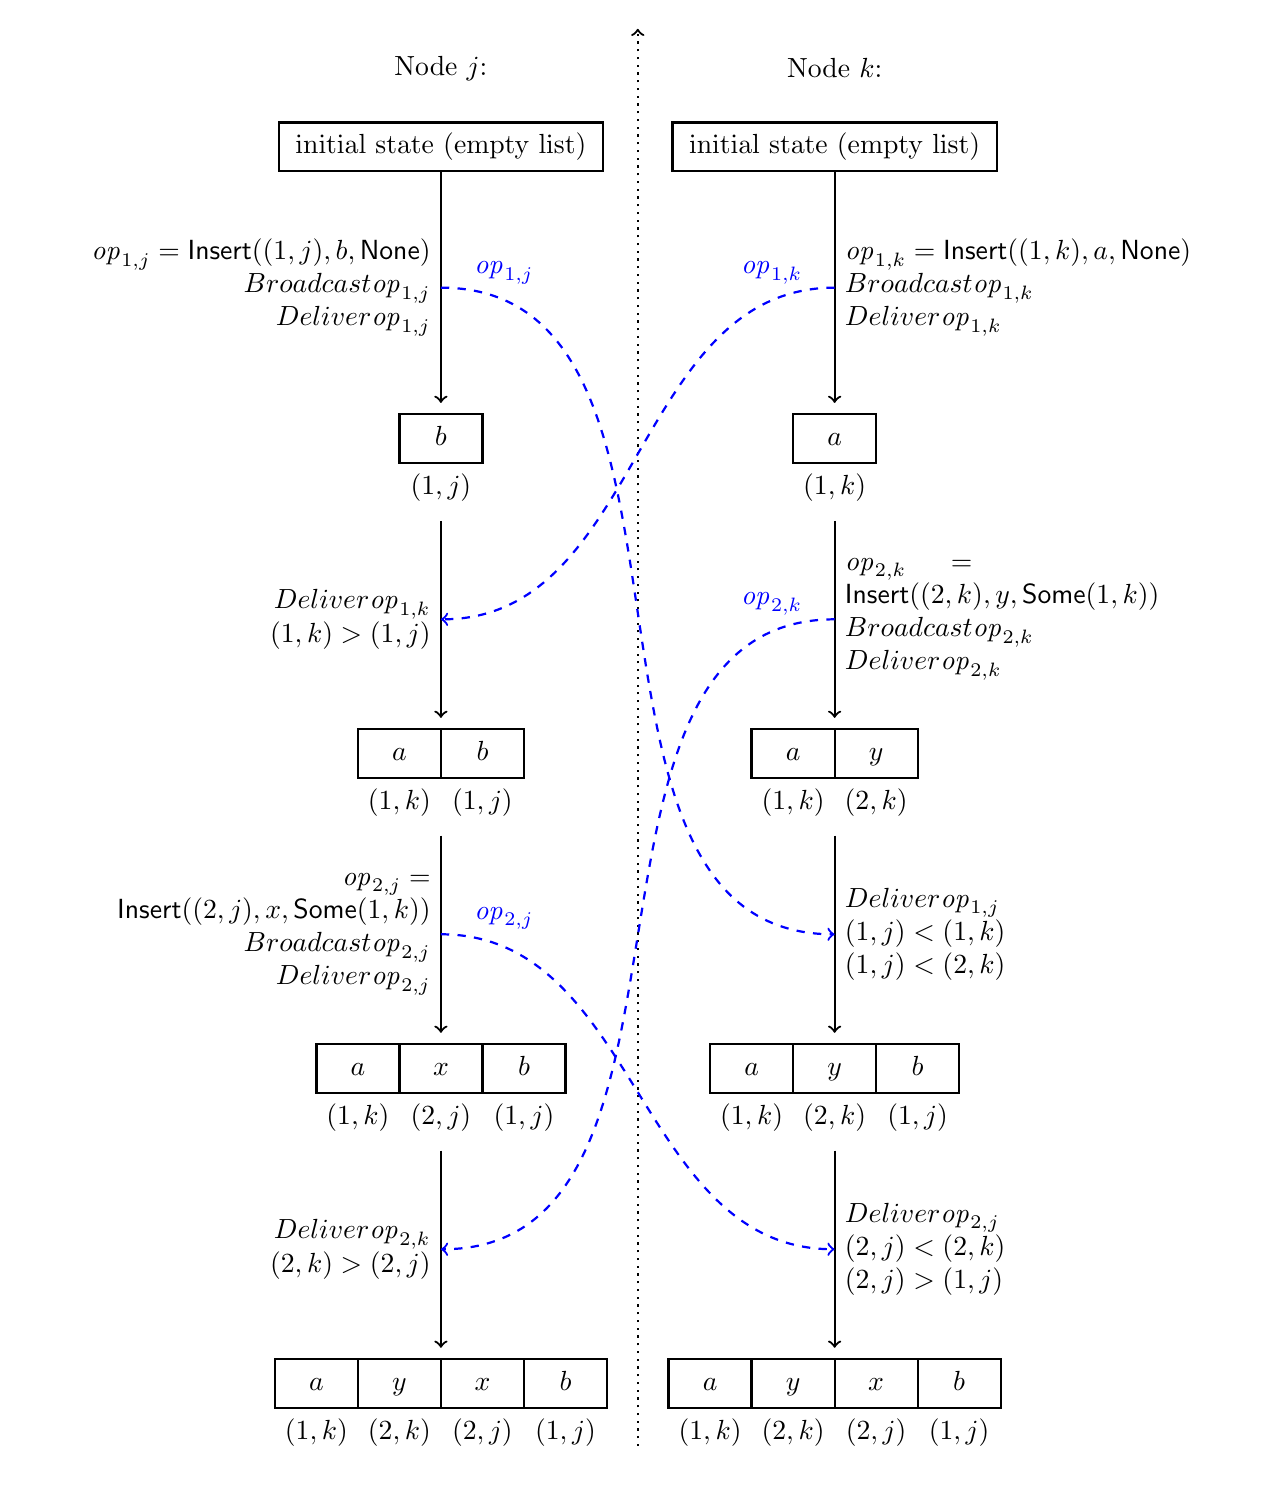
\begin{tikzpicture}[auto,scale=1.0]
\onehalfspacing
\path [draw,dotted] (2.5,-0.5) -- (2.5,17.5);

\tikzstyle{initstate}=[rectangle,draw,inner xsep=6pt,text height=8pt,text depth=3pt]
\tikzstyle{state}=[matrix,column sep={30pt,between origins}]
\tikzstyle{val}=[draw,anchor=base,minimum width=30pt,text height=8pt,text depth=3pt]
\tikzstyle{oid}=[anchor=base]
\tikzstyle{leftevent}=[left,text width=5cm,text ragged left,midway]
\tikzstyle{rightevent}=[right,text width=5cm,text ragged,midway]
\tikzstyle{every path}=[thick,->]

\node (leftR) at (0,17) {Node $j$:};
\node (left1) at (0,16) [initstate] {initial state (empty list)};
\node (left2) at (0,12) [state] {
    \node [val] {$b$};     \\
    \node [oid] {$(1,j)$}; \\
};
\node (left3) at (0,8) [state] {
    \node [val] {$a$};     & \node [val] {$b$};     \\
    \node [oid] {$(1,k)$}; & \node [oid] {$(1,j)$}; \\
};
\node (left4) at (0,4) [state] {
    \node [val] {$a$};     & \node [val] {$x$};     & \node [val] {$b$};     \\
    \node [oid] {$(1,k)$}; & \node [oid] {$(2,j)$}; & \node [oid] {$(1,j)$}; \\
};
\node (left5) at (0,0) [state] {
    \node [val] {$a$};     & \node [val] {$y$};     & \node [val] {$x$};     & \node [val] {$b$};     \\
    \node [oid] {$(1,k)$}; & \node [oid] {$(2,k)$}; & \node [oid] {$(2,j)$}; & \node [oid] {$(1,j)$}; \\
};

\draw (left1) -- (left2) node (send1j) [leftevent] {
    \hfill $\mathit{op}_{1,j} = \mathsf{Insert}((1, j), b, \mathsf{None})$ \\
    \hfill $\text{Broadcast } \mathit{op}_{1,j}$ \\
    \hfill $\text{Deliver } \mathit{op}_{1,j}$ \\
};
\draw (left2) -- (left3) node (recv1k) [leftevent] {
    \hfill $\text{Deliver } \mathit{op}_{1,k}$ \\
    \hfill $(1,k) > (1,j)$ \\
};
\draw (left3) -- (left4) node (send2j) [leftevent] {
    \hfill $\mathit{op}_{2,j} = \mathsf{Insert}((2, j), x, \mathsf{Some}(1,k))$ \\
    \hfill $\text{Broadcast } \mathit{op}_{2,j}$ \\
    \hfill $\text{Deliver } \mathit{op}_{2,j}$ \\
};
\draw (left4) -- (left5) node (recv2k) [leftevent] {
    \hfill $\text{Deliver } \mathit{op}_{2,k}$ \\
    \hfill $(2,k) > (2,j)$ \\
};

\node (rightR) at (5,17) {Node $k$:};
\node (right1) at (5,16) [initstate] {initial state (empty list)};
\node (right2) at (5,12) [state] {
    \node [val] {$a$};     \\
    \node [oid] {$(1,k)$}; \\
};
\node (right3) at (5,8) [state] {
    \node [val] {$a$};     & \node [val] {$y$};     \\
    \node [oid] {$(1,k)$}; & \node [oid] {$(2,k)$}; \\
};
\node (right4) at (5,4) [state] {
    \node [val] {$a$};     & \node [val] {$y$};     & \node [val] {$b$};     \\
    \node [oid] {$(1,k)$}; & \node [oid] {$(2,k)$}; & \node [oid] {$(1,j)$}; \\
};
\node (right5) at (5,0) [state] {
    \node [val] {$a$};     & \node [val] {$y$};     & \node [val] {$x$};     & \node [val] {$b$};     \\
    \node [oid] {$(1,k)$}; & \node [oid] {$(2,k)$}; & \node [oid] {$(2,j)$}; & \node [oid] {$(1,j)$}; \\
};

\draw (right1) -- (right2) node (send1k) [rightevent] {
    $\mathit{op}_{1,k} = \mathsf{Insert}((1, k), a, \mathsf{None})$ \\
    $\text{Broadcast } \mathit{op}_{1,k}$ \\
    $\text{Deliver } \mathit{op}_{1,k}$ \\
};
\draw (right2) -- (right3) node (send2k) [rightevent] {
    $\mathit{op}_{2,k} = \mathsf{Insert}((2, k), y, \mathsf{Some}(1, k))$ \\
    $\text{Broadcast } \mathit{op}_{2,k}$ \\
    $\text{Deliver } \mathit{op}_{2,k}$ \\
};
\draw (right3) -- (right4) node (recv1j) [rightevent] {
    $\text{Deliver } \mathit{op}_{1,j}$ \\
    $(1,j) < (1,k)$ \\
    $(1,j) < (2,k)$ \\
};
\draw (right4) -- (right5) node (recv2j) [rightevent] {
    $\text{Deliver } \mathit{op}_{2,j}$ \\
    $(2,j) < (2,k)$ \\
    $(2,j) > (1,j)$ \\
};

\begin{scope}[dashed,blue]
    \tikzstyle{every node}=[text centered]
    \draw (send1j.east) to [out=0,in=180] (recv1j.west);
    \draw (send2j.east) to [out=0,in=180] (recv2j.west);
    \draw (send1k.west) to [out=180,in=0] (recv1k.east);
    \draw (send2k.west) to [out=180,in=0] (recv2k.east);
    \node at (0.8,14.4) {$\mathit{op}_{1,j}$};
    \node at (0.8, 6.2) {$\mathit{op}_{2,j}$};
    \node at (4.2,14.4) {$\mathit{op}_{1,k}$};
    \node at (4.2,10.2) {$\mathit{op}_{2,k}$};
\end{scope}
\end{tikzpicture}

\caption{RGA example}\label{fig.two-lists}
\end{figure}


\begin{figure}[t]
  \raggedright
  \begin{isabellebody}
\isanewline
\isacommand{theorem}\isamarkupfalse%
\ \ convergence{\isacharcolon}\isanewline
\ \ \isakeyword{assumes}\ {\isachardoublequoteopen}set\ xs\ {\isacharequal}\ set\ ys{\isachardoublequoteclose}\isanewline
\ \ \ \ \ \ \ \ \ \ {\isachardoublequoteopen}concurrent{\isacharunderscore}ops{\isacharunderscore}commute\ xs{\isachardoublequoteclose}\isanewline
\ \ \ \ \ \ \ \ \ \ {\isachardoublequoteopen}concurrent{\isacharunderscore}ops{\isacharunderscore}commute\ ys{\isachardoublequoteclose}\isanewline
\ \ \ \ \ \ \ \ \ \ {\isachardoublequoteopen}distinct\ xs{\isachardoublequoteclose}\isanewline
\ \ \ \ \ \ \ \ \ \ {\isachardoublequoteopen}distinct\ ys{\isachardoublequoteclose}\isanewline
\ \ \ \ \ \ \ \ \ \ {\isachardoublequoteopen}hb{\isacharunderscore}consistent\ xs{\isachardoublequoteclose}\isanewline
\ \ \ \ \ \ \ \ \ \ {\isachardoublequoteopen}hb{\isacharunderscore}consistent\ ys{\isachardoublequoteclose}\isanewline
\ \ \isakeyword{shows}\ \ \ {\isachardoublequoteopen}apply{\isacharunderscore}operations\ xs\ {\isacharequal}\ apply{\isacharunderscore}operations\ ys{\isachardoublequoteclose}\isanewline
%
\isacommand{using}\isamarkupfalse%
\ assms\ \isacommand{proof}\isamarkupfalse%
{\isacharparenleft}induction\ xs\ arbitrary{\isacharcolon}\ ys\ rule{\isacharcolon}\ rev{\isacharunderscore}induct{\isacharcomma}\ simp{\isacharparenright}\isanewline
\ \ \isacommand{case}\isamarkupfalse%
\ assms{\isacharcolon}\ {\isacharparenleft}snoc\ x\ xs{\isacharparenright}\isanewline
\ \ \isacommand{then}\isamarkupfalse%
\ \isacommand{obtain}\isamarkupfalse%
\ prefix\ suffix\ \isakeyword{where}\ ys{\isacharunderscore}split{\isacharcolon}\ {\isachardoublequoteopen}ys\ {\isacharequal}\ prefix\ {\isacharat}\ x\ {\isacharhash}\ suffix\ {\isasymand}\ concurrent{\isacharunderscore}set\ x\ suffix{\isachardoublequoteclose}\isanewline
\ \ \ \ \isacommand{using}\isamarkupfalse%
\ hb{\isacharunderscore}consistent{\isacharunderscore}prefix{\isacharunderscore}suffix{\isacharunderscore}exists\ \isacommand{by}\isamarkupfalse%
\ fastforce\isanewline
\ \ \isacommand{moreover}\isamarkupfalse%
\ \isacommand{hence}\isamarkupfalse%
\ {\isacharasterisk}{\isacharcolon}\ {\isachardoublequoteopen}distinct\ {\isacharparenleft}prefix\ {\isacharat}\ suffix{\isacharparenright}{\isachardoublequoteclose}\ {\isachardoublequoteopen}hb{\isacharunderscore}consistent\ xs{\isachardoublequoteclose}\isanewline
\ \ \ \ \isacommand{using}\isamarkupfalse%
\ assms\ \isacommand{by}\isamarkupfalse%
\ auto\isanewline
\ \ \isacommand{moreover}\isamarkupfalse%
\ \isacommand{{\isacharbraceleft}}\isamarkupfalse%
\isanewline
\ \ \ \ \isacommand{have}\isamarkupfalse%
\ {\isachardoublequoteopen}hb{\isacharunderscore}consistent\ prefix{\isachardoublequoteclose}\ {\isachardoublequoteopen}hb{\isacharunderscore}consistent\ suffix{\isachardoublequoteclose}\isanewline
\ \ \ \ \ \ \isacommand{using}\isamarkupfalse%
\ ys{\isacharunderscore}split\ assms\ hb{\isacharunderscore}consistent{\isacharunderscore}append{\isacharunderscore}D{\isadigit{2}}\ hb{\isacharunderscore}consistent{\isacharunderscore}append{\isacharunderscore}elim{\isacharunderscore}ConsD\ \isacommand{by}\isamarkupfalse%
\ blast{\isacharplus}\isanewline
\ \ \ \ \isacommand{hence}\isamarkupfalse%
\ {\isachardoublequoteopen}hb{\isacharunderscore}consistent\ {\isacharparenleft}prefix\ {\isacharat}\ suffix{\isacharparenright}{\isachardoublequoteclose}\isanewline
\ \ \ \ \ \ \isacommand{by}\isamarkupfalse%
\ {\isacharparenleft}metis\ assms{\isacharparenleft}{\isadigit{8}}{\isacharparenright}\ hb{\isacharunderscore}consistent{\isacharunderscore}append\ hb{\isacharunderscore}consistent{\isacharunderscore}append{\isacharunderscore}porder\ list{\isachardot}set{\isacharunderscore}intros{\isacharparenleft}{\isadigit{2}}{\isacharparenright}\ ys{\isacharunderscore}split{\isacharparenright}\isanewline
\ \ \isacommand{{\isacharbraceright}}\isamarkupfalse%
\isanewline
\ \ \isacommand{moreover}\isamarkupfalse%
\ \isacommand{have}\isamarkupfalse%
\ {\isacharasterisk}{\isacharasterisk}{\isacharcolon}\ {\isachardoublequoteopen}concurrent{\isacharunderscore}ops{\isacharunderscore}commute\ {\isacharparenleft}prefix\ {\isacharat}\ suffix\ {\isacharat}\ {\isacharbrackleft}x{\isacharbrackright}{\isacharparenright}{\isachardoublequoteclose}\isanewline
\ \ \ \ \isacommand{using}\isamarkupfalse%
\ assms\ ys{\isacharunderscore}split\ \isacommand{by}\isamarkupfalse%
\ {\isacharparenleft}clarsimp\ simp{\isacharcolon}\ concurrent{\isacharunderscore}ops{\isacharunderscore}commute{\isacharunderscore}def{\isacharparenright}\isanewline
\ \ \isacommand{moreover}\isamarkupfalse%
\ \isacommand{hence}\isamarkupfalse%
\ {\isachardoublequoteopen}concurrent{\isacharunderscore}ops{\isacharunderscore}commute\ {\isacharparenleft}prefix\ {\isacharat}\ suffix{\isacharparenright}{\isachardoublequoteclose}\isanewline
\ \ \ \ \isacommand{by}\isamarkupfalse%
\ {\isacharparenleft}force\ simp\ del{\isacharcolon}\ append{\isacharunderscore}assoc\ simp\ add{\isacharcolon}\ append{\isacharunderscore}assoc{\isacharbrackleft}symmetric{\isacharbrackright}{\isacharparenright}\isanewline
\ \ \isacommand{ultimately}\isamarkupfalse%
\ \isacommand{have}\isamarkupfalse%
\ {\isachardoublequoteopen}apply{\isacharunderscore}operations\ xs\ {\isacharequal}\ apply{\isacharunderscore}operations\ {\isacharparenleft}prefix{\isacharat}suffix{\isacharparenright}{\isachardoublequoteclose}\isanewline
\ \ \ \ \isacommand{using}\isamarkupfalse%
\ assms\ \isacommand{by}\isamarkupfalse%
\ simp\ {\isacharparenleft}metis\ Diff{\isacharunderscore}insert{\isacharunderscore}absorb\ Un{\isacharunderscore}iff\ {\isacharasterisk}\ concurrent{\isacharunderscore}ops{\isacharunderscore}commute{\isacharunderscore}appendD\ set{\isacharunderscore}append{\isacharparenright}\isanewline
\ \ \isacommand{moreover}\isamarkupfalse%
\ \isacommand{have}\isamarkupfalse%
\ {\isachardoublequoteopen}apply{\isacharunderscore}operations\ {\isacharparenleft}prefix{\isacharat}suffix\ {\isacharat}\ {\isacharbrackleft}x{\isacharbrackright}{\isacharparenright}\ {\isacharequal}\ apply{\isacharunderscore}operations\ {\isacharparenleft}prefix{\isacharat}x\ {\isacharhash}\ suffix{\isacharparenright}{\isachardoublequoteclose}\isanewline
\ \ \ \ \isacommand{using}\isamarkupfalse%
\ ys{\isacharunderscore}split\ assms\ {\isacharasterisk}{\isacharasterisk}\ concurrent{\isacharunderscore}ops{\isacharunderscore}commute{\isacharunderscore}concurrent{\isacharunderscore}set\ \isacommand{by}\isamarkupfalse%
\ force\isanewline
\ \ \isacommand{ultimately}\isamarkupfalse%
\ \isacommand{show}\isamarkupfalse%
\ {\isacharquery}case\isanewline
\ \ \ \ \isacommand{using}\isamarkupfalse%
\ ys{\isacharunderscore}split\ \isacommand{by}\isamarkupfalse%
\ {\isacharparenleft}force\ simp{\isacharcolon}\ append{\isacharunderscore}assoc{\isacharbrackleft}symmetric{\isacharbrackright}\ simp\ del{\isacharcolon}\ append{\isacharunderscore}assoc{\isacharparenright}\isanewline
\isacommand{qed}\isamarkupfalse%
  \end{isabellebody}
  \caption{Proof of convergence theorem in Isar.}
  \label{fig.convergence}
\end{figure}
